\documentclass{scrartcl}

\usepackage{
    microtype,
    polyglossia,
    xltxtra,
    amsmath,
    mathtools,
    scrlayer-scrpage,
    dsfont,
    amssymb,
    xcolor,
    blindtext,
    marvosym,
    tikz,
    fontspec,
    mathrsfs,
    pgfplots,
    booktabs,
    tabularx,
    multirow,
    stubs
}

\pagenumbering{gobble}

%Matrix settings
\setcounter{MaxMatrixCols}{20}

%Font settings
\setsansfont{Linux Biolinum O}
\setmainfont{Linux Libertine O}

%subsection font
\setkomafont{section}{\LARGE\bfseries\rmfamily}
\setkomafont{subsection}{\Large\bfseries\rmfamily}
\addtokomafont{disposition}{\rmfamily}

\setmainlanguage{german}

%Tables
\newcolumntype{L}{>{\raggedright\arraybackslash}X}%
\newcolumntype{C}{>{\centering\arraybackslash}X}%
\newcolumntype{R}{>{\raggedleft\arraybackslash}X}%

\title{Brain Inspired Computing (SS 19): Sheet 5}
\author{Sven Bordukat, Paul Meehan, Juan Tomás Morales}
\date{}

\begin{document}
    \maketitle
    \section*{Exercise 1}
    \begin{itemize}
        \item[a)] Assume that $N$ is the number of spikes generated by a Poisson process in the interval $[0,T]$, then $ p_T(N=1) = \nu Te^{-\nu T} $ is the probability for exactly one spike to occur during this time, and $ p_\text{ISI}(t_1) = \nu e^{-\nu t_1} $ is the probability this spike occuring at $t_1$. Using this and Bayes theorem we obtain
        \begin{align*}
            p(t_1|N=1) &= \frac{p(N=1|t_1)p_\text{ISI}(t_1)}{p_T(N=1)} \\
            &= \frac{(p_{T-t_1}(N=0))\cdot \nu e^{-\nu t_1}}{\nu Te^{-\nu T}} \\
            &= \frac{e^{-\nu(T - t_1)}\cdot e^{\nu(T - t_1)}}{T} = \frac{1}{T}.
        \end{align*}
        \item[b)] Given a Poisson process that generates $N$ spikes over an interval $T$ with the ISI distribution $p_\text{ISI}(s) = \nu e^{-\nu s}$, the mean of the ISI distribution is $$ \int_0^{\infty} \nu se^{-\nu s}ds = \nu^{-1}. $$ Therefore, we have on average $T/\nu^{-1} = \nu T$ spikes over an interval of $T$. Hence, we have $E[N] = \nu T$ and by virtue of the Poisson distribution $p_T(N) = \frac{(\nu T)^N}{N!}e^{-\nu T}$, i.e., $\nu$ is the rate of the Poisson process.
        \item[c)] Given two random variables $N_1$ and $N_2$, that are both Poisson distributed with $p_T(N_1;\nu_1)$ and $p_T(N_2;\nu_2)$, the sum of these variables $N=N_1+N_2$ is distributed according to \begin{align*}
            p_T(N=j,\nu) &= \sum_{k=0}^j p_T(k;\nu_1)p_T(j-k;\nu_2) \\
            &= \sum_{k=0}^j \frac{(\nu_1 T)^k}{k!}e^{-\nu_1 T}\frac{(\nu_2 T)^{j-k}}{(j-k)!}e^{-\nu_2 T} \\
            &= e^{-(\nu_1+\nu_2)T}\sum_{k=0}^j \frac{1}{j!}\frac{j!}{k!(j-k)!}(\nu_1T)^k(\nu_2T)^{j-k} \\
            &= \frac{(\nu_1+\nu_2 T)^j}{j!}e^{-(\nu_1+\nu_2) T}
        \end{align*}
        and we see that $\nu = \nu_1+\nu_2$, for the last step we used the Binomial theorem, $k,j\in\mathds N$.
        \item[d)] For the poisson process we have the mean given by
        \begin{align*}
            \text{E}[N] &= \sum_{N=0}^\infty N\frac{(\nu T)^N}{N!}e^{-\nu T} \\
            &= \sum_{N=1}^\infty N\frac{(\nu T)^N}{N!}e^{-\nu T} \\
            &= \sum_{N=1}^\infty \nu T\frac{(\nu T)^{N-1}}{(N-1)!}e^{-\nu T} \\
            &= \nu Te^{-\nu T} \sum_{N=0}^\infty \frac{(\nu T)^{N}}{N!} \\
            &= \nu Te^{-\nu T}e^{\nu T} \\
            &= \nu T.
        \end{align*}
        The variance can be derived using $\text{Var}[N] = \text{E}[N^2] - \text{E}[N]^2$, we have
        \begin{align*}
            \text{E}[N^2] &= \sum_{N=0}^\infty N^2\frac{(\nu T)^N}{N!}e^{-\nu T} \\
            &= \sum_{N=1}^\infty N^2\frac{(\nu T)^N}{N!}e^{-\nu T} \\
            &= \sum_{N=1}^\infty \nu TN\frac{(\nu T)^{N-1}}{(N-1)!}e^{-\nu T} \\
            &= \nu Te^{-\nu T} \left(\left(\sum_{N=0}^\infty \frac{(\nu T)^{N}}{N!}\right)+\nu T\left(\sum_{N=0}^\infty \frac{(\nu T)^{N}}{N!}\right)\right) \\
            &= \nu Te^{-\nu T}\left(e^{\nu T}+\nu Te^{\nu T}\right) \\
            &= \nu T + \nu^2T^2
        \end{align*}
        and, therefore, $\text{Var}[N] = \nu T + \nu^2T^2 - \nu^2T^2 = \nu T$.
        \item[e)] The coefficient of variation is $\text{CV}_\text{ISI} = \frac{\sqrt{\text{Var}[s]}}{\text{E}[s]} $ and we have
        \begin{align*}
            \text{E}[s] &= \int_{0}^\infty \nu se^{-\nu s}ds \\
            &= \int_0^\infty e^{-\nu s} ds \\
            &= 1/\nu
        \end{align*}
        as well as
        \begin{align*}
            \text{E}[s^2] &= \int_{0}^\infty \nu s^2e^{-\nu s}ds \\
            &= \int_0^\infty se^{-\nu s} ds \\
            &= \text{E}[s]/\nu \\
            &= 1/\nu^2
        \end{align*}
        and we therefore have $\text{CV}_\text{ISI} = \frac{\sqrt{1/\nu^2}}{1/\nu} = 1$.
    \end{itemize}
    
    \newpage
    \section*{Exercise 2}
    \begin{figure}[h]
        \label{bins}
            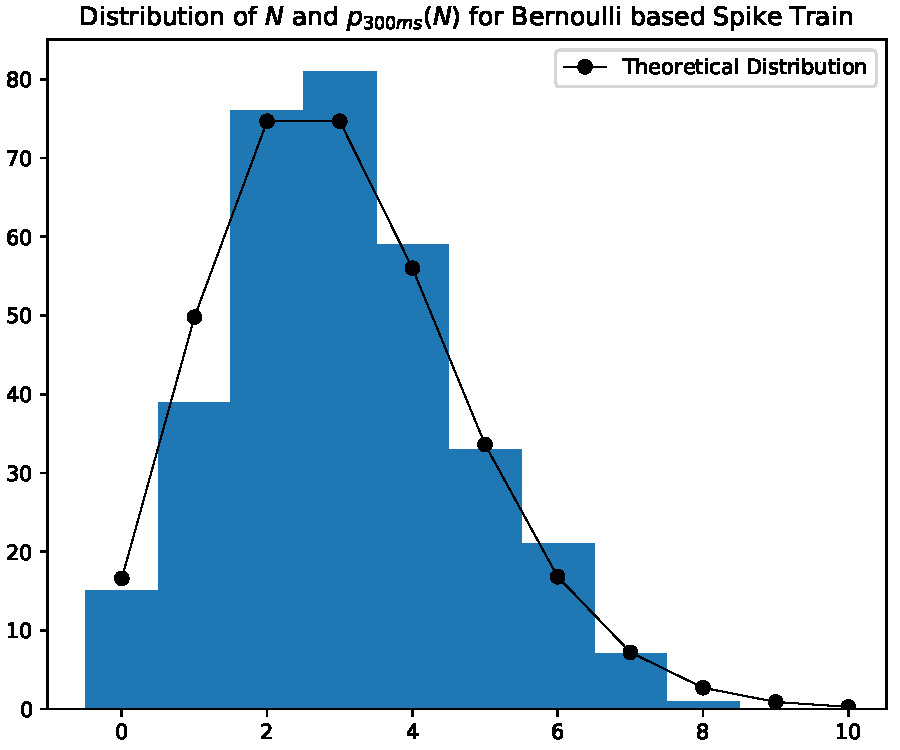
\includegraphics[width=0.5\linewidth]{spikes_dist_bin.pdf}
            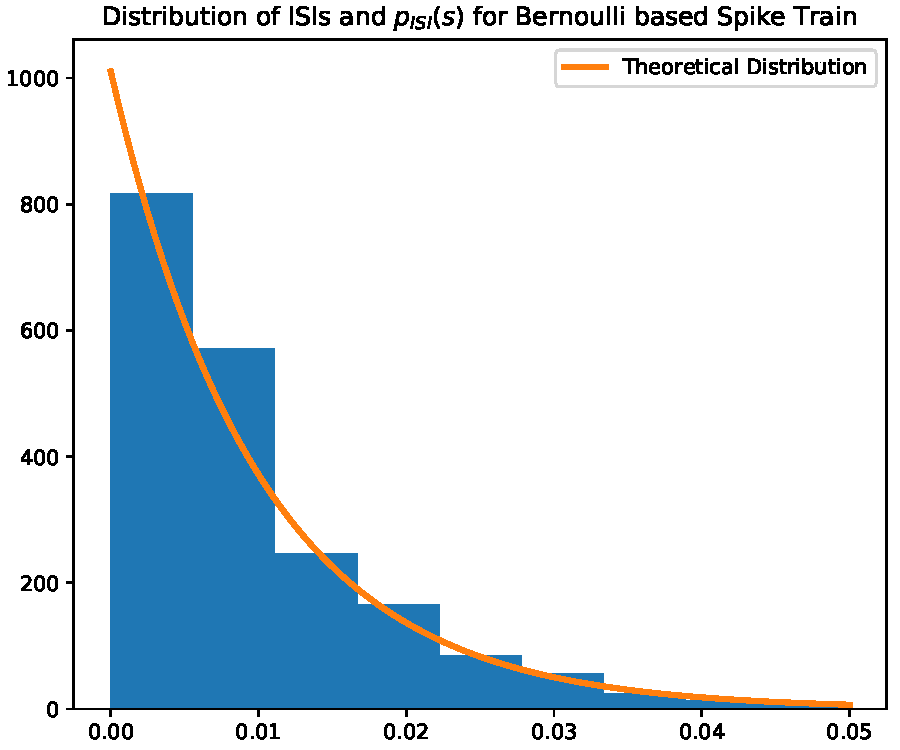
\includegraphics[width=0.5\linewidth]{isi_dist_bin.pdf}
            \caption{Plots of the ISIs distribution and the distribution of spike numbers in 300ms intervals for the approach from a).}
    \end{figure}
    \begin{figure}[h]
        \label{isi}
        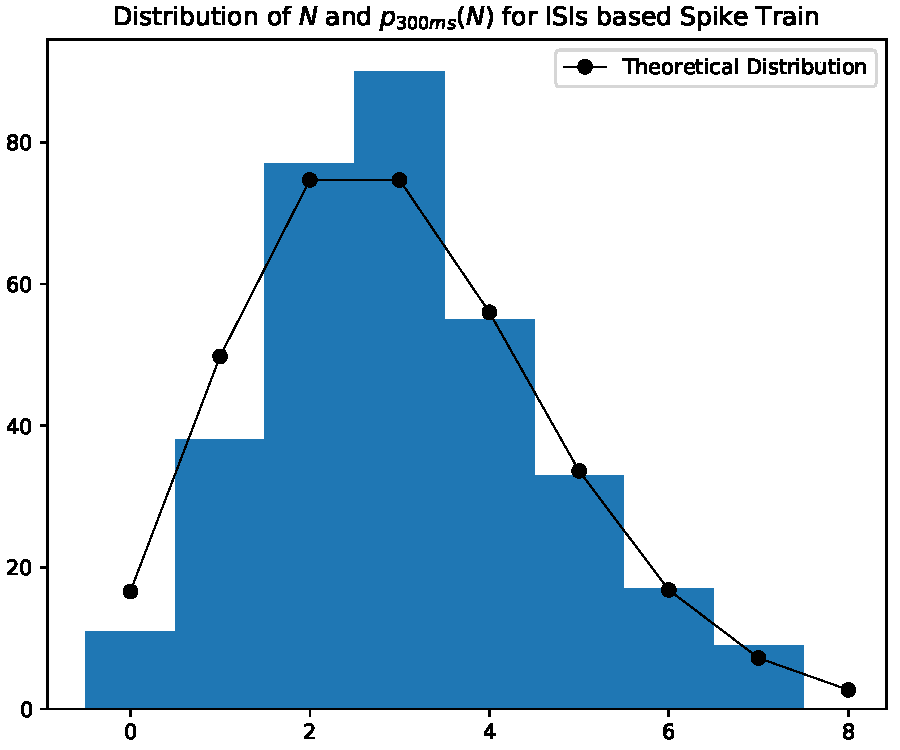
\includegraphics[width=0.5\linewidth]{spikes_dist_isi.pdf}
        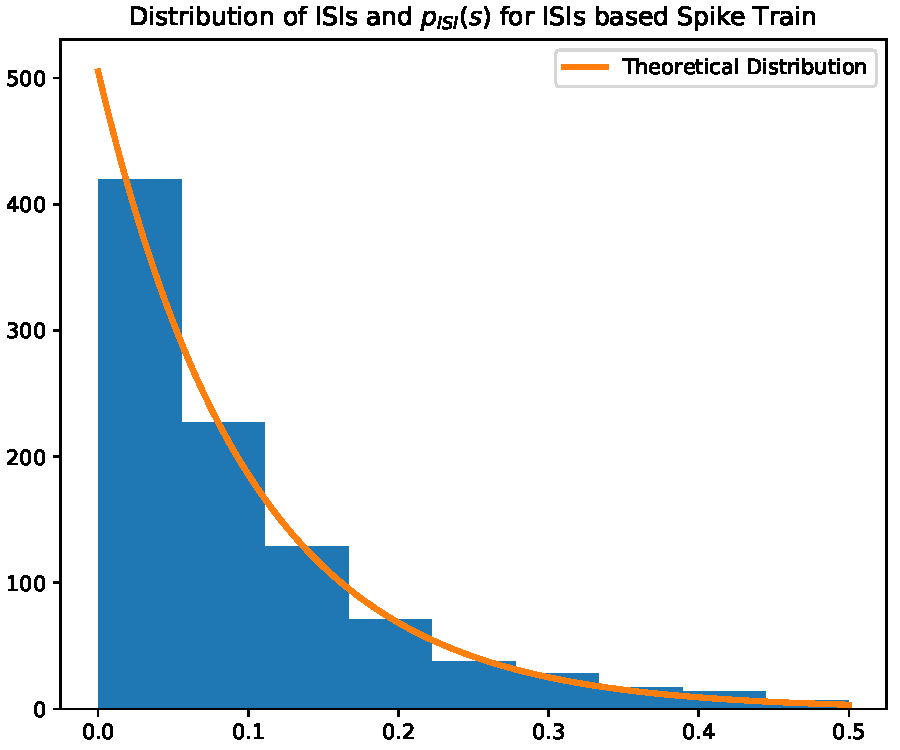
\includegraphics[width=0.5\linewidth]{isi_dist_isi.pdf}
        \caption{Plots of the ISIs distribution and the distribution of spike numbers in 300ms intervals for the approach from b).}
    \end{figure}
    \begin{figure}[h]
        \label{uni}
        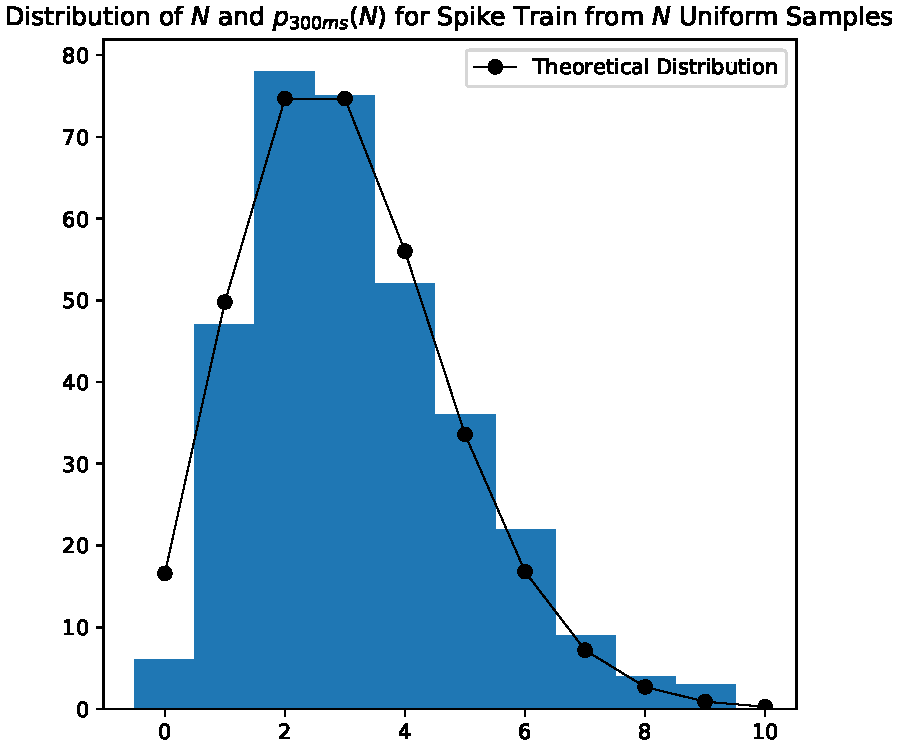
\includegraphics[width=0.5\linewidth]{spikes_dist_uni.pdf}
        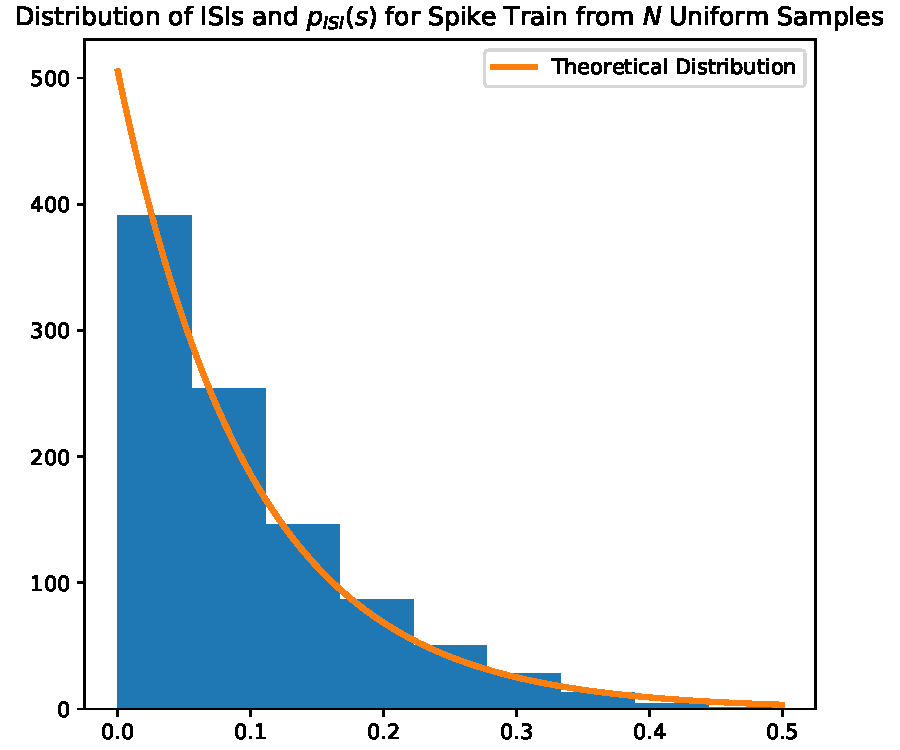
\includegraphics[width=0.5\linewidth]{isi_dist_uni.pdf}
        \caption{Plots of the ISIs distribution and the distribution of spike numbers in 300ms intervals for the approach from c).}
    \end{figure}
    \pagebreak
    \section*{Exercise 3}
    \begin{itemize}
        \item[a)] Empirically, $\nu_i$ is determined to be $\nu_i=3788Hz$.
    \item[b)] \begin{align*}
        t_{eff}&=\frac{C_m}{g_{tot}}=\frac{C_m}{g_{exc}+g_{inh}+C_m/\tau_m}\\
    w^e_{syn}&=w_0^e*(E_{exc}-u)=0.45\\
    w^i_{syn}&=w_0^i*(E_{inh}-u)=-0.5\\
\end{align*}
\begin{figure}[h]
    \centering
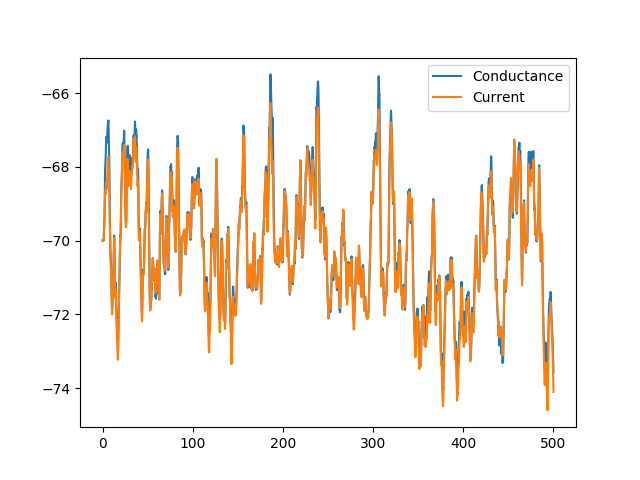
\includegraphics[width=0.8\textwidth]{trace_0.png}
    \caption{Membrane potential trace of COBA and CUBA neurons}
\end{figure}
\item[c)] See figure \ref{hist0}
\begin{figure}[h]
    \centering
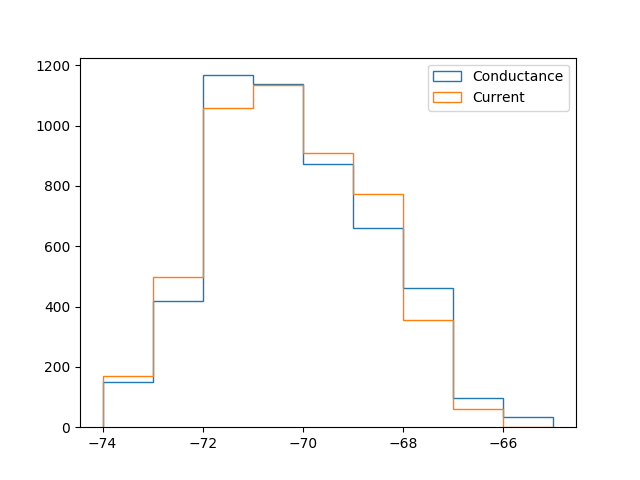
\includegraphics[width=0.8\textwidth]{hist_0.png}
    \caption{Histogram of COBA and CUBA neuron membrane potential}
    \label{hist0}
\end{figure}
        \item[d)] In the HCS case, we see that for the COBA neuron
        there is a slightly larger count of potentials in the central ($-70mV$) region
        as for the CUBA neuron. Furthermore, the bins for the COBA neuron extend
        further along the x-axis, up to about $-62mV$. The latter can be explained by
        viewing the very beginning of the experiment, when the potential jumps up
        rapidly through excitation, without giving the inhibitory neuron a ``chance
        to respond''. In the CUBA case, as everything is based on currents, the jump
        is much less rapid.
        \begin{figure}[h]
            \centering
        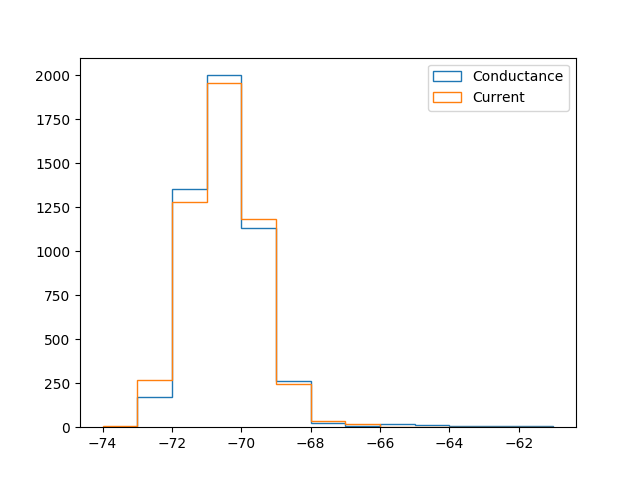
\includegraphics[width=0.8\textwidth]{hist_5.png}
            \caption{Histogram of COBA and CUBA neuron membrane potential in the HCS case}
        \end{figure}
    \end{itemize}

\end{document}
